\documentclass[11pt,a4paper]{article}
\usepackage[utf8]{inputenc}
\usepackage[T1]{fontenc}
\usepackage{ae}
\usepackage{mathtools}
\usepackage{amsfonts,amsmath,amssymb,amsthm}
\usepackage[libertine,cmintegrals,cmbraces,vvarbb]{newtxmath}
\usepackage[english]{babel}
\usepackage{cancel}
\usepackage{enumerate}
\usepackage[pdftex]{graphicx}
\usepackage{float}
\usepackage{caption}
\usepackage{subcaption}
\usepackage{listings}
\usepackage{fancyhdr}
\pagestyle{fancy}
\usepackage{fancybox}
\usepackage[dvipsnames]{xcolor}
\usepackage{tikz}
\usetikzlibrary{matrix,arrows,decorations.pathmorphing}
\usepackage{verbatim}
\usepackage{marvosym}
\usepackage{algorithm2e}
\usepackage{todonotes}
\usepackage{color}
\usepackage{bm}
\usepackage{todonotes}

\makeatletter
\newcommand\todoname{todo}
\newcommand\listtodoname{List of todos}
\newcommand\listoftodos{%
  \section*{\listtodoname}\@starttoc{tod}}
\makeatother

\setlength{\parindent}{0em}

\newcommand{\F}[0]{\mathbb{F}}
\newcommand{\N}[0]{\mathbb{N}}
\newcommand{\Z}[0]{\mathbb{Z}}
\newcommand{\Q}[0]{\mathbb{Q}}
\newcommand{\R}[0]{\mathbb{R}}
\newcommand{\C}[0]{\mathbb{C}}
\newcommand{\B}[0]{\mathbb{B}}
\newcommand{\im}[0]{\mathit{i}}
\newcommand{\uber}[2]{{{#1} \choose {#2}}}
\newcommand{\vect}[1]{\begin{pmatrix}#1\end{pmatrix}}
\newcommand{\norm}[1]{\left\lvert #1 \right\rvert}

\def\students{Willi Gierke, Arik Elimelech, Mehmed Halilovic, Leon Sixt}

\fancyhead[L]{SS 2017}
\fancyhead[C]{Maschinelles Lernen 2}
\fancyhead[R]{Assignment 08 -- \textbf{ESHG}}
\fancyfoot[L]{}
\fancyfoot[C]{\students}
\fancyfoot[R]{}


\title{Maschinelles Lernen 1 -- Group ESHA \\
        Assignment 01
}

\author{\students}
\date{\today}

\begin{document}
\maketitle

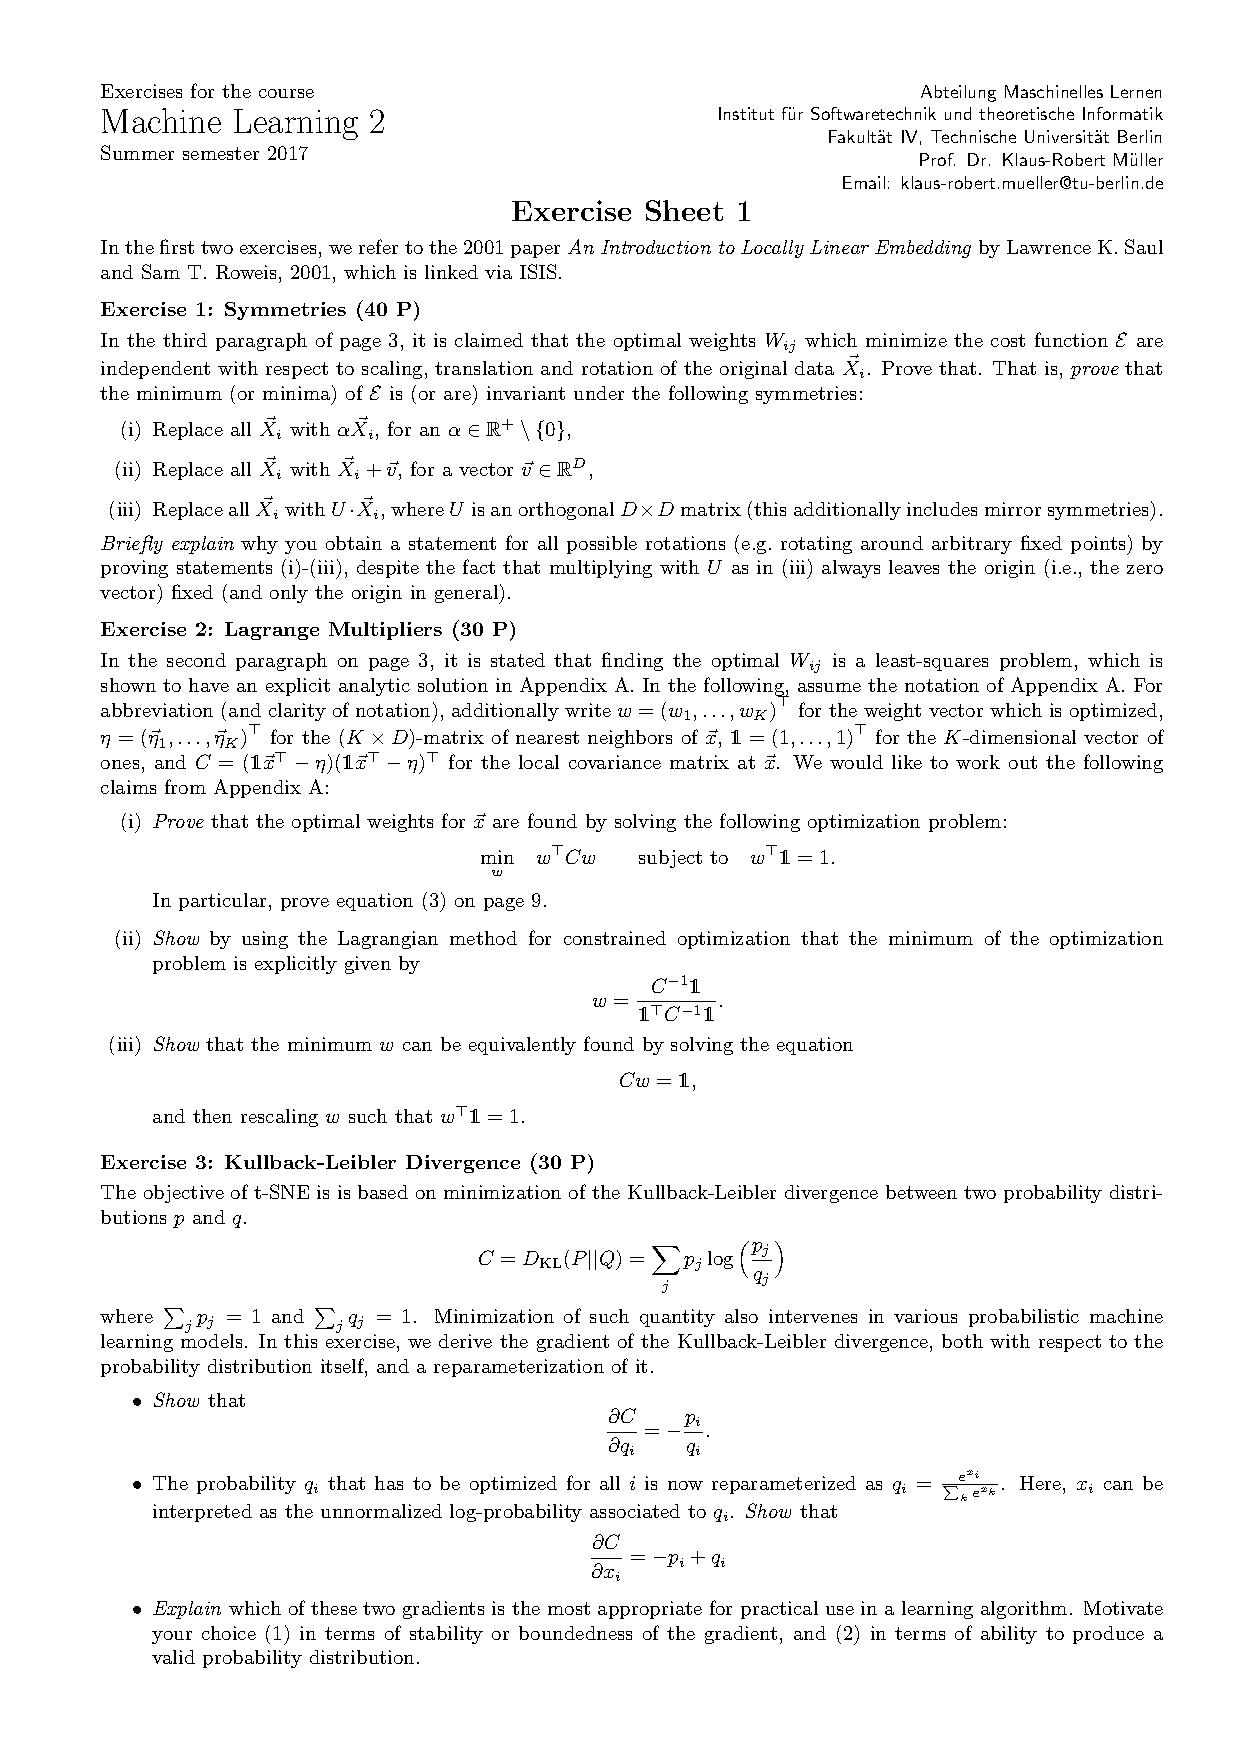
\includegraphics[clip, trim=0.5cm 0.5cm 0.5cm 5cm, width=1.00\textwidth]{sheet01.pdf}

\listoftodos
\clearpage

\section*{1}

\subsection*{i}

\begin{gather*}
\epsilon(W) = \sum_{i} |\vec{X_{i}} - \sum_j W_{ij} \vec{X_{j}}| ^{2} \\
\tilde{\epsilon}(W) = \sum_{i} |\alpha \vec{X_{i}} - \sum_j W_{ij} \alpha \vec{X_{j}}| ^{2} \\
\tilde{\epsilon}(W) = \sum_{i} |\alpha (\vec{X_{i}} - \sum_j W_{ij} \vec{X_{j}})| ^{2} \\
\tilde{\epsilon}(W) = \sum_{i} \alpha^2 |(\vec{X_{i}} - \sum_j W_{ij} \vec{X_{j}})| ^{2} \\
\tilde{\epsilon}(W) = \alpha^2 \sum_{i} |(\vec{X_{i}} - \sum_j W_{ij} \vec{X_{j}})| ^{2} \\
\end{gather*}

Since $\alpha^2$ in $\tilde{\epsilon}(W)$ does not influence the weights of the maximum we get the same result as in ${\epsilon}(W)$

\subsection*{ii}

\begin{gather*}
\epsilon(W) = \sum_{i} |\vec{X_{i}} - \sum_j W_{ij} \vec{X_{j}}| ^{2} \\
\tilde{\epsilon}(W) = \sum_{i} |(\vec{X_{i}} + \vec{v}) - \sum_j W_{ij}  (\vec{X_{j}} + \vec{v})| ^{2} \\
\tilde{\epsilon}(W) = \sum_{i} |(\vec{X_{i}} + \vec{v}) - (\sum_j W_{ij} \vec{X_{j}}) - (\sum_j W_{ij} \vec{v}))| ^{2} \\
\tilde{\epsilon}(W) = \sum_{i} |(\vec{X_{i}} + \vec{v}) - (\sum_j W_{ij} \vec{X_{j}}) - \vec{v} (\sum_j W_{ij}))| ^{2} \\
\tilde{\epsilon}(W) = \sum_{i} |\vec{X_{i}} + \vec{v} - (\sum_j W_{ij} \vec{X_{j}}) - \vec{v}| ^{2} \\
\tilde{\epsilon}(W) = \sum_{i} |\vec{X_{i}} - (\sum_j W_{ij} \vec{X_{j}})| ^{2} = \epsilon(W)
\end{gather*}

\subsection*{iii}

\begin{gather*}
\epsilon(W) = \sum_{i} |\vec{X_{i}} - \sum_j W_{ij} \vec{X_{j}}| ^{2} \\
\tilde{\epsilon}(W) = \sum_{i} |U\vec{X_{i}} - \sum_j W_{ij} U\vec{X_{j}}| ^{2} \\
\tilde{\epsilon}(W) = \sum_{i} |U\vec{X_{i}} - U(\sum_j W_{ij} \vec{X_{j}})| ^{2} \\
\tilde{\epsilon}(W) = \sum_{i} |U(\vec{X_{i}} - \sum_j W_{ij} \vec{X_{j}})| ^{2}
\end{gather*}
We can treat $(\vec{X_{i}} - \sum_j W_{ij} \vec{X_{j}})$ as a vector and then we get $\tilde{\epsilon}(W) = \epsilon(W)$, since:
\begin{gather*}
|U\vec{v}|^2 = <U\vec{v}, U\vec{v}> = <\vec{v}, U^T U\vec{v}> = <\vec{v}, \vec{v}> = |\vec{v}|^2
\end{gather*}

We get rotation around arbitrary points by combining translation and rotation. If we want to rotate around point $A$, we can first do a translation so that point $A$ becomes the center. Then we rotate in the center and after that we reverse the translation.

\section*{2}

\subsection*{i}

\begin{gather*}
\epsilon = |\vec{x}  - \sum_j w_j \vec{\eta_j}|^2 \\
\epsilon = |\sum_j w_j \vec{x} -  \sum_j w_j \vec{\eta_j}|^2 \\
\epsilon = |\sum_j w_j (\vec{x} - \vec{\eta_j})|^2 \\
\epsilon = (\sum_j w_j (\vec{x} - \vec{\eta_j})) (\sum_k w_k (\vec{x} - \vec{\eta_k})) \\
\epsilon = \sum_j \sum_k w_j w_k  (\vec{x} - \vec{\eta_j}) (\vec{x} - \vec{\eta_k}) \\
\epsilon = \sum_{j,k} w_j w_k C_{j,k} \\
\epsilon = \sum_j w_j \sum_k C_{j,k} w_k \\
\epsilon = \sum_j w_j (C w_k)_k
\end{gather*}
where $(C w_k)_k = \sum_j C_{k,j} w_j$
\begin{gather*}
\epsilon = \vec{w}^TC\vec{w} \\
\end{gather*}

\todo[inline]{Finish this task}

\subsection*{ii}

\begin{gather*}
L(w,\lambda) = w^T Cw + \lambda(w^T 1 - 1) \\
\frac{\partial L}{\partial \lambda} = w^T  -1 \\
\frac{\partial L}{\partial w_i} = \frac{\partial}{\partial w_i} \\
\end{gather*}
\todo[inline]{Mathbbm is not working}
\todo[inline]{Finish this task}
\subsection*{iii}

\todo[inline]{Finish this task}

\section*{3}

\begin{gather*}
C = \sum_j p_j log(\frac{p_j}{q_j}) \\
\frac{\partial C}{\partial q_i} = p_i * \frac{\partial}{\partial q_i} log(\frac{p_i}{q_i}) \\
\frac{\partial C}{\partial q_i} = p_i * \frac{q_j}{p_j} * (-\frac{p_i}{q_i^2}) \\
\frac{\partial C}{\partial q_i} = -\frac{p_i}{q_i} \\
\end{gather*}

\todo[inline]{Finish this task}

\end{document}
